\section{Conifold eigenlines and changes of choices}
\label{sec:eigenlines-choices}

\subsection{Two simple lines on the full domain}

Put $c=w_f/w_g>0$. The finite characteristic
polynomial is
\begin{equation}\label{eq:conifold-characteristic}
 256\mu^2-36(w_f+w_g)\mu+5w_fw_g=0.
\end{equation}
Its roots are $\mu_\pm=w_g\kappa_\pm(c)$, where
\begin{equation}\label{eq:conifold-ratio-roots}
 \kappa_\pm(c)=
 \frac{9(c+1)\pm\sqrt{81(c-1)^2+4c}}{128}.
\end{equation}
Since
$81(c-1)^2+4c-(c+1)^2=80(c-1)^2$,
\begin{equation}\label{eq:uniform-conifold-gap}
 0<\mu_-/\mu_+\le\frac45,\qquad
             \mu_+-\mu_-\ge\frac15\mu_+.
\end{equation}
Thus the finite lines are relatively separated
throughout the positive quadrant. The actual
relative eigenvalue estimate makes both actual
positive eigenvalues simple for all sufficiently
small admissible $p$, uniformly in $c$.
Lemma~\ref{lem:relative-subspace-transport}
then gives
\begin{equation}\label{eq:conifold-line-transport}
 \|P^M_{\mathcal A\ell_\pm(p)}
                 -P^M_{L_\pm(p)}\|_M\le Ce(p)\to0,
\end{equation}
where $\ell_\pm$ are the actual real eigenlines
and $L_\pm$ the generalized finite eigenlines.
No sign for an eigenvector is chosen.

An exact expression is
\begin{equation}\label{eq:conifold-line-formula}
 L_\pm=\RR(4\mu_\pm,\ 36\mu_\pm-5w_f).
\end{equation}
The vector is nonzero and satisfies
$(E_p-\mu_\pm M)x=0$. For $c\to\infty$,
\begin{equation}\label{eq:conifold-large-ratio}
 \begin{aligned}
 \mu_+&\sim\frac9{64}w_f,&
 \mu_-&\sim\frac5{36}w_g,\\
 L_+&\longrightarrow\RR(1,1/9),&
 L_-&\longrightarrow\RR(0,1).
 \end{aligned}
\end{equation}
For $c\to0$ the roles reverse:
\[
 \mu_+\sim\frac9{64}w_g,\quad
 \mu_-\sim\frac5{36}w_f,\qquad
 L_+\to\RR(1/9,1),\quad L_-\to\RR(1,0).
\]
For $c\to c_0\in(0,\infty)$ both have scale
$w_g$, with constants $\kappa_\pm(c_0)$
and the corresponding distinct finite lines.
At $c=1$ the lines are $\RR(1,-1)$ and
$\RR(1,1)$, with coefficients $1/8$ and
$5/32$, respectively.

The boundary filtration for $c\to\infty$
has slow subspace $\RR g$ and its
$M$-orthogonal fast complement
$\RR(1,1/9)$. These are exactly the
successive-kernel spaces in
Theorem~\ref{thm:fixed-map-hierarchy}.
A path with no ratio limit need not
have a limiting filtration; the
pointwise statement
\eqref{eq:conifold-line-transport}
still applies.

\begin{figure}[tb]
 \centering
 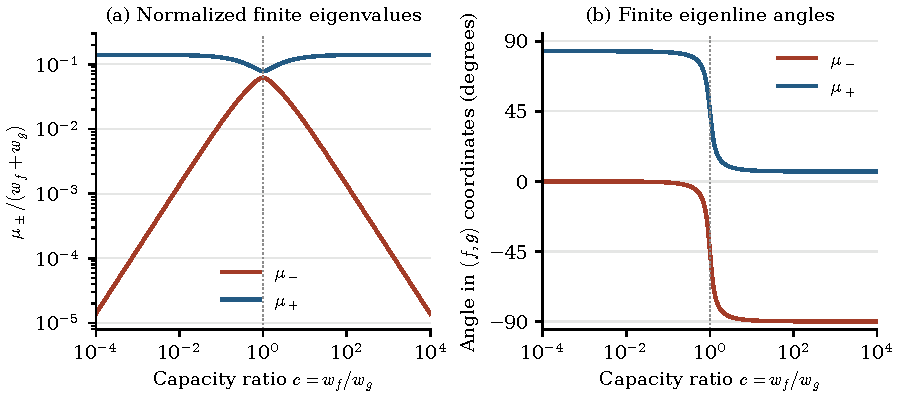
\includegraphics[width=\textwidth]{output/figures/finite_pair.pdf}
 \caption{The finite pair $(\operatorname{diag}(c,1),M)$, with quotient mass $M$.
 Left: its generalized eigenvalues divided by $1+c$.
 Right: the angles of eigenline representatives with positive
 first coordinate in the displayed $(f,g)$ basis.
 The dotted line marks equal capacities.}
 \label{fig:finite-pair}
\end{figure}

\subsection{Realized logarithmic hierarchies}

For positive functions $F(h),G(h)\to\infty$,
the admissible slice
\begin{equation}\label{eq:general-exponential-slice}
 p(h)=(a,a,a,-3a;\ b,b,b,-3b),\qquad
                  a=e^{-F(h)},\quad b=e^{-G(h)}
\end{equation}
eventually belongs to $B^\circ$.
The bounded holomorphic units and the
factor $-3$ change each logarithm by a
bounded amount. Hence
\[
 w_f\sim\frac{8\pi}{F(h)},\qquad
 w_g\sim\frac{8\pi}{G(h)}.
\]
If $F/G\to0$, the actual simple
eigenvalues satisfy
\begin{equation}\label{eq:actual-general-hierarchy}
 \lambda_+\sim\frac{9\pi}{8F(h)},\qquad
 \lambda_-\sim\frac{10\pi}{9G(h)}.
\end{equation}
Taking $F=h^{-1}$, $G=h^{-2}$ gives
the constants in \eqref{eq:separated-spectrum-intro}.
Taking $G=h^{-1}\log(1/h)$ instead gives
the orders $h$ and $h/\log(1/h)$;
taking $G=h^{-1}\log\log(1/h)$ gives
$h$ and $h/\log\log(1/h)$. These are
paths on the actual family; they are
not holomorphic arcs at the origin.
This completes the eigenline and path
consequences announced after
Theorem~\ref{thm:main}.

\subsection{Fixed cutoffs and exterior identifications}

Keep $W,M$ fixed, but choose two compact
central exteriors $C_1,C_2$ with their
central-metric closed projections and
cohomology maps. Let $\mathcal A_1,
\mathcal A_2$ be the resulting observers.
Choose a larger compact exterior $C$
containing both, and set $\zeta=\Pi_Cu$.
The class of this closed form agrees
on both smaller exteriors, so
$\mathcal A_1\zeta=\mathcal A_2\zeta$.
The first-order projection estimate gives
\begin{equation}\label{eq:fixed-cutoff-discrepancy}
 \|(\mathcal A_2-\mathcal A_1)u\|_M
       \le C\|\dd u\|_{L^2(C,g_p)}.
\end{equation}
Here the actual and central exterior
metrics are uniformly equivalent.
The constants may depend on these fixed
choices.

On $S_p$, put
$B_p=\mathcal A_2(\mathcal A_1|_{S_p})^{-1}$
and $\sigma_p=\max\Eig(E_p,M)$.
Equation \eqref{eq:fixed-cutoff-discrepancy}
and the mass and energy estimates show
that $\mathcal A_2$ is also invertible
for small $p$, and
\begin{equation}\label{eq:cutoff-relative-transport}
 \begin{aligned}
 \|B_p-I\|_M&\le C\sqrt{\sigma_p},\\
 \sqrt{E_p((B_p-I)x)}
       &\le C\sqrt{\sigma_p}\sqrt{E_p(x)}.
 \end{aligned}
\end{equation}
For the second line, use
$E_p(y)\le\sigma_pM(y)$ and
$q_p(\mathcal A_1^{-1}x)\le(1+o(1))E_p(x)$.
The first follows from the cluster bound
$q_p\le C\sigma_p\|\cdot\|^2$.
The triangle inequality in the energy
seminorm gives
\[
 (1-C\sqrt{\sigma_p})E_p
       \le B_p^*E_pB_p
       \le(1+C\sqrt{\sigma_p})E_p,
\]
after changing $C$, and the mass obeys
the analogous estimate. The observed
forms transform exactly as
$B_p^*Q_{2,p}B_p=Q_{1,p}$ and
$B_p^*N_{2,p}B_p=N_{1,p}$.
Thus both observers give the same
relative description without a
lower bound on the eigenvalue ratio.

The same conclusion holds when exterior
identifications differ by a smooth isotopy
preserving the relevant exterior, with
uniform derivative, inverse-Jacobian and
generating-vector-field bounds.
The homotopy formula reads
$F_1^*u-F_0^*u=\dd Ku+K\dd u$.
The observation of the exact term is
zero, and the other term is bounded
by $C\|\dd u\|$. Density extends the
argument to form-domain inputs.
An arbitrary shrinking cutoff or
unbounded isotopy requires another
estimate. Phase interpolations supported
in the necks leave the fixed exterior
observer unchanged.

\subsection{Coordinates, polarization and base change}

Under a finite coordinate change $x=Sx'$,
the data transform as
\[
 E'=S^*ES,\qquad M'=S^*MS,\qquad
                       \mathcal A'=S^{-1}\mathcal A.
\]
Generalized eigenvalues and intrinsic
relative inequalities are unchanged,
and subspaces are transported by $S$.
No Euclidean condition-number bound on
$S$ is needed. An integral marking
change must preserve the specified
lattice; this observation does not
supply a lattice from spectral data.

A permitted analytic node-coordinate
change has the form
$\tau'_i=u_i(p)\tau_{\pi(i)}$,
with holomorphic units bounded above
and away from zero. Transport the
link generators by their signs and
permutation. Then
\[
 |\log|\tau'_i||=|\log|\tau_{\pi(i)}||+O(1),
\]
so $E'_p$ and $E_p$ differ relatively
by $O(L_{\min}^{-1})$. This follows
term by term from the reciprocal
lengths and the nonnegative period
squares. The geometric mass transforms
by congruence.
Lemma~\ref{lem:relative-subspace-transport}
and \eqref{eq:uniform-conifold-gap}
give an $O(L_{\min}^{-1})$ change of
the transported finite eigenlines.

Polarization is genuine geometric
input. Scaling the Kähler class by
a fixed $c>0$ scales the Ricci-flat
metric by $c$. In real dimension six
the two-form squared $L^2$ norm scales
by $c$, whereas its $\dd$-energy
scales by one. The eigenvalues
therefore scale by $c^{-1}$.

For a holomorphic base map with
$\tau_i(s)=a_is^{\nu_i}+O(s^{\nu_i+1})$,
$a_i\ne0$ and $\nu_i>0$,
\begin{equation}\label{eq:holomorphic-arc-capacity}
 \frac{2\pi}{|\log|\tau_i(s)||}
       \sim\frac{2\pi}{\nu_i|\log|s||}.
\end{equation}
All capacities have one logarithmic
order. A ramification $s=v^m$ multiplies
every $\nu_i$ by $m$ and divides the
leading coefficients expressed in
$|\log|v||$ by $m$. This reparametrizes
fibres; it does not preserve a
coefficient in a fixed parameter.
For an admissible monomial map
$\tau_i(z)=u_i(z)\prod_jz_j^{a_{ij}}$,
the corresponding length is
$\sum_ja_{ij}|\log|z_j||+O(1)$.
Such a map must factor through the
actual relation base and smooth
the selected nodes. Eight arbitrarily
prescribed monomials need not do so.
